\chapter{Spielgerät und Zubehör}
\label{tisch}


%%%%%%%%%%%%%%%%%%%%%%%%%%%%%%%%%%%%%%%%%%%%%%
\section{Der Tisch}
\label{tisch:tisch}

Der Tisch zusammen mit einem Ball ist das Spielgerät beim Tischfußball. 
Das etwa 1,1 m lange und 0,7 m breite Spielfeld ist im Tischkorpus, der auf vier Beinen steht, eingelassen und von Banden umrundet. An den Stirnseiten sind die Tore platziert, die mit einer Torauffangschale oder einem Ballrücklauf ausgestattet sind.  
Die jeweils 11 Spielfiguren sind auf 4 Stangen (für drei Spielbereiche) verteilt:
\begin{itemize}  
\item die Torwartstange, auch Torwart (\gls{abwehr}) 
\item die 2er-Stange, auch die Zwei (\gls{abwehr}) 
\item die 5er-Stange, auch die Fünf (\gls{mittelfeld})
\item die 3er-Stange (\gls{sturm})
\end{itemize}  
Die Stangen können mittels Griffen vor- und zurückgedreht und rein- und rausgeschoben werden.
Wenn man am Tisch steht, ist die Spielrichtung von links nach rechts, also das linke Tor ist das eigene und das rechte Tor das vom Gegner.
Neben diesem Grundaufbau gibt es viele Unterschiede bei den vielen \nameref{tisch:tisch:modelle}n. 

\subsection{Tischmodelle}
\label{tisch:tisch:modelle}

Inzwischen gibt es Tischmodelle vieler Hersteller in allen Qualitäts- und Preis-Kategorien:
\begin{itemize}
\item günstige, aber auch billige Tische gibt es schon ab 100 Euro 
\item qualitiative Tische für Hobbyspieler gibt es ab 300-600 Euro
\item Trainingstische für Turnierspieler gibt es ab 600-1.200 Euro
\item offizieller Turniertische gibt es ab 1.200 Euro 
\end{itemize}

Letztendlich sollte der Tisch dem Spielniveau angemessen sein, damit der Spielspaß hochgehalten wird. Dennoch gibt es ein paar Grundsätze, die man beispielsweise bei einem Tischkauf beachten sollte:
\begin{itemize}
\item Der Korpus sollte ein gewisses Gewicht haben, damit er nicht leicht verrutscht. Turniertische beispielsweise wiegen über 100 kg.
\item Die Beine sollten nicht wackeln und höhenverstellbar sein.
\item Die Stangen sollten sich nicht leicht verbiegen lassen.
\item {\bf Empfehlung:} Bei einer Anschaffung eines Tisches und von Bällen sollte man darauf achten, dass ein griffiges Ball-Handling von Vorteil für das Erlernen von einem kontrollierten Spiel ist.
\end{itemize}

In Tabelle \ref{tab:tische} werden die Merkmale der 5 offiziellen Tischmodelle des \gls{itsf} und der zwei weiteren Partnertische des \gls{dtfb} verglichen. In der Tabelle wird Bezug auf das jeweilige offizielle Turniermodell genommen, jedoch hat jeder dieser Tischhersteller Modelle für das Anfänger, Jugend- oder Hobbyspieler.    

{\small
\begin{center} 
\begin{table} 
\begin{tabular}{ p{1.5cm}||p{2cm}|p{2cm}|p{2cm}|p{2cm}|p{2cm}} 
 	& Figuren & Spielfläche & Tore & Griffe & Region \\ 
\hline 
\hline 
Leonhart (DTFB, ITSF) & Soccer (Plastik) & hart (Plastik) und normalen Banden & 20 cm breit & rund (Gummi) & Deutschland und Nachbarländer \\ 
\hline 
Ullrich  (DTFB) &  Soccer (Plastik) &  hart (Plastik) und normalen Banden & 20,5 cm breit & 10-kantig (Gummi) & Deutschland \\ 
\hline 
Lettner (DTFB)  & Soccer (Plastik)  &  hart (Plastik) und normalen Banden & ??? & ??? & Deutschland \\ 
\hline 
Bonzini (DTFB, ITSF)  & schwerer Fuss (Metall) & weich (Linoleum) und normalen Banden & ??? & keilförmig (Plastik), wechselbar & Frankreich und Nord-Europa \\ 
\hline 
Garlando (ITSF)  & schmal, Soccer-ähnlich (Plastik) &  hart (Glass) und schrägen Banden & ??? & rund (Plastik und Holz) & Österreich und Südost-Europa \\ 
\hline 
Roberto (ITSF) & quaderförmig (Plastik) &  hart (Plastik) und normalen Banden & ??? & rund (Gummi) & Italien und Südost-Europa \\ 
\hline 
Tornado (ITSF)  & keilförmig (Plastik) &  hart (Plastik) und normalen Banden & 20 cm breit & 6-kantig (Holz oder Gummi) & Nordamerika und englischsprachige Länder \\ 
\end{tabular} 
%\caption{Offizielle \gls{dtfb} und \gls{itsf} Tische mit ihren Eigenheiten. [\cite{www:kickerbau}, \cite{www:tischfussball-online}]}
\label{tab:tische}
\end{table} 
\end{center}
}



%%%%%%%%%%%%%%%%%%%%%%%%%%%%%%%%%%%%%%%%%%%%%%
\subsection{Standort}
\label{tisch:tisch:standort}




Ein Tisch sollte genügend Platz für den Tisch selbst und die Spieler bei voll ausgezogene Stangen haben. Ein Tisch ist  0,75 m x 1,5 m groß und braucht daher eine etwa 2 m x 2,5 m große Fläche (Abb. \ref{fig:tisch:platzbedarf}).

Zudem sollte der Tisch auf einem stabilen und relativ geraden Boden stehen. Bekommt ein Tisch einen neuen Standort, sollte er ausgerichtet werden. Mit Hilfe einer Wasserwaage oder an Hand des Rollen des Balls kann man die Spielfläche durch Höhenrvrstellen der Beine gerade ausrichten (Abb. \ref{fig:tisch:ausrichten}). Dann sollte der Ball ruhig liegenbleiben, wenn man diesen irgendwo auf das Spielfeld legt.

\begin{figure}
%\begin{wrapfigure}{r}{0.6\textwidth} 
\centering 
\begin{subfigure}[b]{0.7\textwidth} 
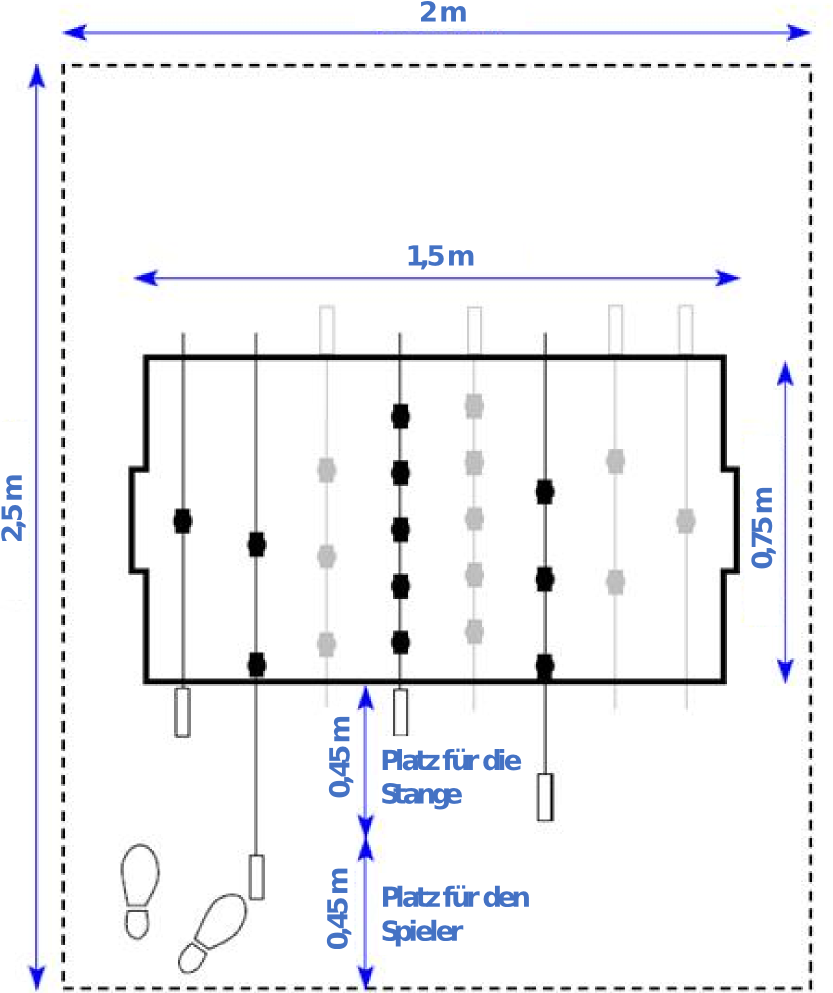
\includegraphics[width=\textwidth]{img/tisch_platzbedarf.png} 
\caption{Platzbedarf} 
\label{fig:tisch:platzbedarf} 
\vspace{0.5cm}
\end{subfigure} 
\begin{subfigure}[b]{0.7\textwidth} 
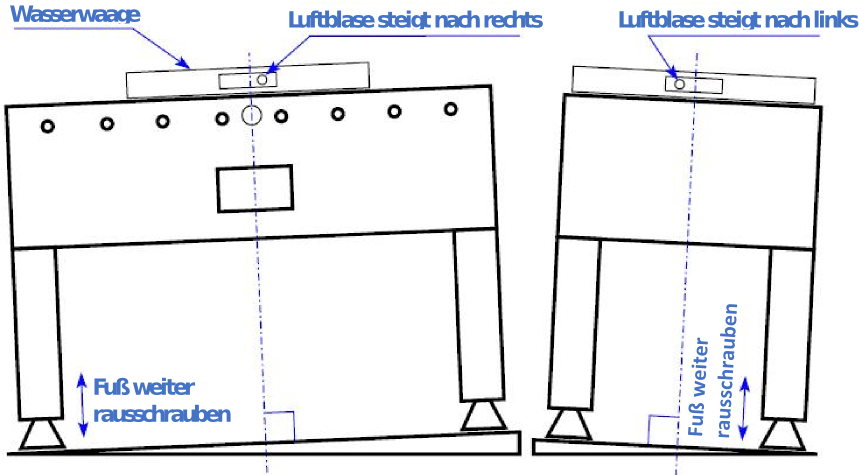
\includegraphics[width=\textwidth]{img/tisch_ausrichten.png} 
\caption{Ausrichten} 
\label{fig:tisch:ausrichten} 
\end{subfigure} 
\label{fig:tisch} 
\caption{Aufstellen eines Tischs [\cite{itsf_basics}]} 
\end{figure}
%\end{wrapfigure}

%%%%%%%%%%%%%%%%%%%%%%%%%%%%%%%%%%%%%%%%%%%%%%
\subsection{Pflege und Wartung}
\label{tisch:tisch:wartung}

Um einen gleichbleibenden Spielspaß zu haben, wird eine regelmäßige Tischpflege und Wartung empfohlen:
\begin{itemize}  
\item {\bf Stangen:} Damit die Stangen leicht laufen, schmieren viele Spieler die Stangen mit Pronto-Spray (Möbelpolitur) oder Silikonöl, bevor Sie Tischfußball spielen. Dabei ist in jedem Fall darauf zu achten, die ganz herausgezogene oder ganz reingeschobenene Stange außerhalb des Tisches und nie über der Spielfläche zu beschmieren. Danach sollten die Stangen hin- und hergedreht werden, während man die Stange rein- und rauszieht, damit sich das Schmiermittel gut über die Stange verteilt  und die Stangen gut in den Lagern laufen.
\item {\bf Spielfeld:} Auf dem Spielfeld sammeln sich über die Zeit Staub, auflösende Gummistückechen vom Puffer oder Ballspuren. Diese lassen sich am einfachsten und schonend mit etwas Glasreiniger und Haushaltspapier entfernen -- zumindest bei Soccer-Spielflächen wie bei Leonhart- oder Ullrich-Tischen. In jedem Fall sollte man auf Spülmittel und Scheuerschwämme verzichten. 
\item {\bf Lager und Puffer:} Das Schmiermittel für die Stangen kann leider auch leicht Staub binden. Diese Masse setzt sich gerne in den Lagern über die Zeit ab. Mit einem zurechtgerollten normalen Schreib-Papier kann man die Ablagerungen durch Durchschieben der Rolle entfernen. Manchmal lohnt sich aber auch eine Grundreinigung und man baut die Figuren, Stangen und Lager aus, um die Lager ohne Stange gründlich zu reinigen. Dabei sollte man sich überlegen, ob man die Puffer ersetzt. Puffer lösen sich durch die Schmiermittel und die Belastung nach einiger Zeit auf.    
\item {\bf Allgemeines:} Natürlich sollten alle Schrauben am Tisch fest sitzen. Es lohnt sich ab und zu zu überprüfen, ob alle Schrauben noch festsitzen.  
\end{itemize}  


%%%%%%%%%%%%%%%%%%%%%%%%%%%%%%%%%%%%%%%%%%%%%%
%%%%%%%%%%%%%%%%%%%%%%%%%%%%%%%%%%%%%%%%%%%%%%
\section{Bälle}
\label{tisch:baelle}

Es gibt verschiedene Typen von Bällen, obwohl der Durchmesser typischerweise 35 mm beträgt -- manchmal auch 34 mm \citep{www:kickerbau:baelle}.
Tischfußball-Bälle unterscheiden sich vor allem in ihrer Griffigkeit und ihrem Gewicht, zudem in ihrer Farbe und auch beim Material.
Insbesondere die Griffigkeit, und damit die Oberflächenbeschaffenheit des Balls, und das Gewicht sind entscheidend für die Spieleigenschaften.  

Vorgestellt werden hier drei Bälle, die auf den Soccertischen (Leonhart, Ullrich, Lettner) üblicherweise gespielt werden und alle aus weißem Plastik sind \citep{www:tfc-reutlingen}:
\begin{itemize}
\item Der Ullrich Ball:
Der Ullrich Ball ist durch seine eher weiche Oberfläche der griffigste Ball unter den Soccer-Bällen. 
Das ermöglicht eine Ballführung mit viel Kontrolle. Insbesondere beim Klemmen kann man damit den Ball an verschiedenen Punkten unter der Stange führen und spielen \ref{klemmen}.
% Grafik ? Foto 
Mit einem üblichen 35 mm Durchmesser wiegt der Ball 24 g.
Dadurch das der Ball relativ weich ist, bekommt mit der Zeit Macken und Dellen, so dass ein langsamer Ball zum Teil nicht mehr ganz gerade rollt.
Er ist offizieller Ball in Deutschland und mit dem DTFB- und dem P4P-Schriftzug bedruckt.
Preis: 2,00 Euro. \\
Spieler: Ab Anfänger bis Profi
\item Der Leonhart Ball: 
Mit einem Durchmesser von 35 mm und einem Gewicht von etwa 27 g ist im Vergleich zu vielen Bällen relativ schwer. 
Zusammen mit seiner harten und doch leicht griffigen Oberfläche hat er damit ruhiges und genaues Rollverhalten.
Er ist mit dem ITSF Schriftzug bedruckt, da er offizeller ITSF Ball für den Leonhart-Tisch ist.
Preis: 2,50 Euro. \\
Spieler: Ab Fortgeschrittener bis Profi
\item Der Lettner Ball (Contus Avant):
Der dritte DTFB zertifizierte Ball ist für den Lettner Tisch entwickelt.
Er hat ein Gewicht von 27 g und einem Durchmesser von 34,9 mm.
Der Ball hat eine harte Oberfläche, ist jedoch leicht griffig. 
Er ist nicht so verbreitet wie der Leonhart- oder Ullrich-Ball. \\
Preis: 2,75 Euro.
Spieler: Ab Amatuer bis Profi
\end{itemize}

Die Griffigkeit hängt nicht nur von der Art des Balls ab, sondern ist ein Zusammenspiel zwischen Figur, Ball und Spieloberfläche. 
Zum Beispiel spielt sich ein Leonhart-Ball auf einem Ullrich-Tisch eher weniger griffig.  
Und auch die offiziellen Tische -- die 5 ITSF- und 3 DTFB-Tische -- haben ihren eigenen zertifizierten Ball und dadurch unterschiedlichste Spieleigenschaften:
Der Bonzini-Ball ist orange und hart, aber auf dem Bonzini-Tisch sehr griffig. 
Im Gegensatz zum Tornado Ball, der aus roten Urethan ist, was in sehr hart und schwer macht -- und sehr ungriffig bzw. rutschig. 



%%%%%%%%%%%%%%%%%%%%%%%%%%%%%%%%%%%%%%%%%%%%%%
\section{Zubehör}
\label{tisch:zubehoer}


\subsection{Griffbänder und Handschuhe}
\label{tisch:zubehoer:griffe}



Hintergrund: Griffwechselsystem

\subsection{Trainingsmaterialien}
\label{tisch:zubehoer:training}
Rodlocks/Gummis, 

Backbouncer

Kickertrainer 

Visual-Kickertrainer (Thomas Hettich):  %https://www.facebook.com/104697842895711/videos/496741320358026/

Foos-Train.com


\subsection{Kleidung und Schuhe}
\label{tisch:zubehoer:kleidung}

Kleidung: Trikots, Schuhe, ...
